\documentclass[12pt]{article}

\usepackage[utf8x]{inputenc} % Включаем поддержку UTF8  
\usepackage[russian]{babel}  % Включаем пакет для поддержки русского языка  
\usepackage{hyperref}        % Для гиперссылок

% Математика
\usepackage{amsmath,amsfonts,amssymb,amsthm,mathtools} % AMS
\usepackage{icomma}
\usepackage{mathrsfs}

\usepackage{xcolor}

% Прога
\usepackage{etoolbox}
\usepackage{listings}

\definecolor{codegreen}{rgb}{0,0.6,0}
\definecolor{codegray}{rgb}{0.5,0.5,0.5}
\definecolor{codepurple}{rgb}{0.58,0,0.82}
\definecolor{backcolour}{rgb}{0.95,0.95,0.92}

\lstdefinestyle{mystyle}{
	backgroundcolor=\color{backcolour},   
	commentstyle=\color{codegreen},
	keywordstyle=\color{magenta},
	numberstyle=\tiny\color{codegray},
	stringstyle=\color{codepurple},
	basicstyle=\ttfamily\footnotesize,
	breakatwhitespace=false,         
	breaklines=true,                 
	captionpos=b,                    
	keepspaces=true,                 
	numbers=left,                    
	numbersep=5pt,                  
	showspaces=false,                
	showstringspaces=false,
	showtabs=false,                  
	tabsize=2
}

\lstset{style=mystyle}

% Цвета
\usepackage{xcolor}

% Картинки
\usepackage{graphicx}
\graphicspath{ {./images/} }

\usepackage{tikzsymbols}

% Работа с таблицами
\usepackage{array,tabularx,tabulary,booktabs} % Дополнительная работа с таблицами
\usepackage{longtable}  % Длинные таблицы
\usepackage{multirow} % Слияние строк в таблице

% Нумерованные списки
\usepackage[shortlabels]{enumitem} % Разные лейблы

% Текст
\usepackage[normalem]{ulem}  % для зачеркивания текста

\newtheorem{property}{Свойство}
\newtheorem{consequence}{Следствие}[property]

\DeclarePairedDelimiter\abs{\lvert}{\rvert}%
\DeclarePairedDelimiter\norm{\lVert}{\rVert}%

% Swap the definition of \abs* and \norm*, so that \abs
% and \norm resizes the size of the brackets, and the 
% starred version does not.
\makeatletter
\let\oldabs\abs
\def\abs{\@ifstar{\oldabs}{\oldabs*}}
%
\let\oldnorm\norm
\def\norm{\@ifstar{\oldnorm}{\oldnorm*}}
\makeatother

\begin{document}
	
	\thispagestyle{empty}
	\begin{center}
		\textbf{ПРАВИТЕЛЬСТВО РОССИЙСКОЙ ФЕДЕРАЦИИ}
		
		\vspace{5ex}
		
		\textbf{Федеральное государственное автономное образовательное учреждение \\ высшего образования \\ <<Национальный исследовательский университет \\ <<Высшая школа экономики>>}
	\end{center}
	\vspace{5ex}
	
	\begin{center}
		Московский институт электроники и математики им. А.Н. Тихонова  
		
		\vspace{5ex}
		
		Департамент прикладной математики
		
		\vspace{10ex}
		\textbf{Отчёт \\ по лабораторной работе №5 \\ по курсу <<Алгоритмизация и программирование>> \\ Задание № 13}
		\vspace{7ex}
		
	\end{center}
	
	\begin{center} 
		\begin{tabular}{| p{0.3\linewidth}| p{0.3\linewidth}| p{0.3\linewidth}|}
			\hline	
			ФИО студента & Номер группы & Дата \\  \hline
			& & \\  
			Кейер Александр \newline Петрович & БПМ-231 & 21.11.2023\\  
			& & \\  \hline		
		\end{tabular}
	\end{center}
	
	\begin{center}
		\vspace{3ex}
		
		\vfill
		
		\normalsize
		
		\textbf{Москва, 2023}
	\end{center}
	
	\newpage
	
	%---------------------------------------------------------------------------------
	
	\section*{Задание (вариант № 13)}
	
	 Дана целочисленная матрица размера $m \cdot n$, где $2 \leq m, n \leq 10$.
	 Программа должна быть разбита на несколько функций и обязательно содержать:
	 \begin{enumerate}
	 	\item функцию формирования исходного массива;
	 	\item функцию вывода исходного массива;
	 	\item одну или более функций, реализующих вычислительную часть алгоритма.
	 \end{enumerate}
	 Все функции должны содержать список параметров, причём адрес массива должен передаваться как параметр функции. Функция main должна содержать только операторы вызова функций. Использовать статический массив. Дополнительных массивов не использовать!
	 \vspace{5pt}
	 \newline
	 \textbf{В строках с чётными элементами на пересечении с главной диагональю найти
	 наибольший нечётный элемент.}
	
	\newpage
	
	\section*{Решение}
	
	\begin{lstlisting}[language=C]
	#include <stdio.h> // Input/output library.
	#include <math.h> // Math library.
	
	const int N = 100;
	
	// Finding pointer on maximum odd element in row function.
	int* findPMaxOddInRow(int arr[][N], int i, int n) {
		int* pMaxOdd = NULL;
		
		for (int j = 0; j < n; j++) {
			if (arr[i][j] % 2 != 0 && (pMaxOdd == NULL || arr[i][j] > *pMaxOdd)) {
				pMaxOdd = &arr[i][j];
			}
		}
		
		return pMaxOdd;
	}
	
	// Function implementing solution.
	int* solution(int arr[][N], int m, int n) {
		int* out = NULL;
		int* pMaxOdd = NULL;
		
		for (int i = 0; i < m; i++) {
			if (arr[i][i] % 2 == 0) {
				pMaxOdd = findPMaxOddInRow(arr, i, n);
				
				if (pMaxOdd != NULL && (out == NULL || *pMaxOdd > *out)) {
					out = pMaxOdd;
				}
			}
		}
		
		return out;
	}
	
	// Array reading function.
	int readArr(int arr[][N], int *pm, int *pn) {
		printf("Enter m >= 2 and n <= 10 numbers: ");
		scanf("%d %d", pm, pn);
		
		for (int i = 0; i < *pm; i++) {
			for (int j = 0; j < *pn; j++) {
				printf("Enter int arr[%d][%d]: ", i, j);
				scanf("%d", &arr[i][j]);
			}
		}
		
		return 0;
	}
	
	// Arrya printing function.
	int printArr(int arr[][N], int m, int n) {
		
		for (int i = 0; i < m; i++) {
			printf("\n");
			
			for (int j = 0; j < n; j++) {
				printf(" %d", arr[i][j]);
			}
		}
		
		return 0;
	}
	
	int main() {
		// Greeting.
		printf("Lab #5 made by Alexander Keyer from BAM231 group.\n\n");
		
		int m, n, arr[N][N];
		
		// Reading array.
		readArr(arr, &m, &n);
		
		// Entered array demonstration.
		printf("\nYou entered this array: ");
		printArr(arr, m, n);
		
		// Get answer.
		int* result = solution(arr, m, n);
		
		printf("\n\n");
		
		// Print answer.
		if (result != NULL) {
			printf("The corresponding answer: %d", *result);
		} else {
			printf("Cannot find corresponding answer.");
		}
		
		return 0;
	}
	\end{lstlisting}
	
	\newpage
	
	\section*{Тесты}
	
	\subsection*{Тест № 1}
	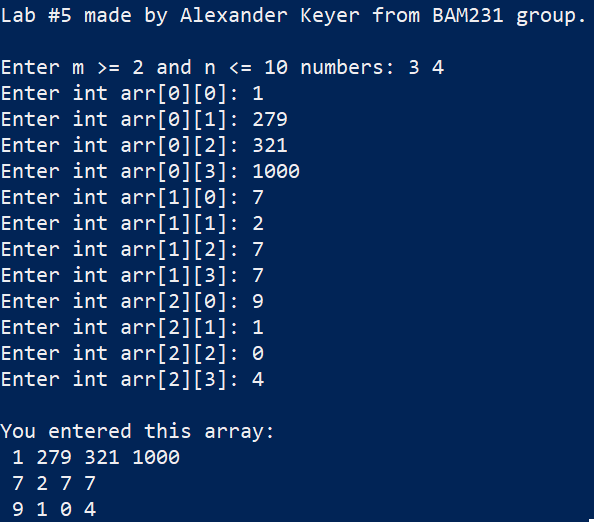
\includegraphics[width=400px]{test_1}
	Программа сработала корректно.
	
	\subsection*{Тест № 2}
	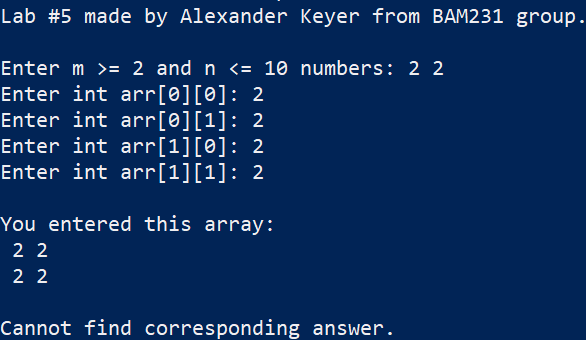
\includegraphics[width=400px]{test_2}
	Программа сработала корректно.
	
	\subsection*{Тест № 3}
	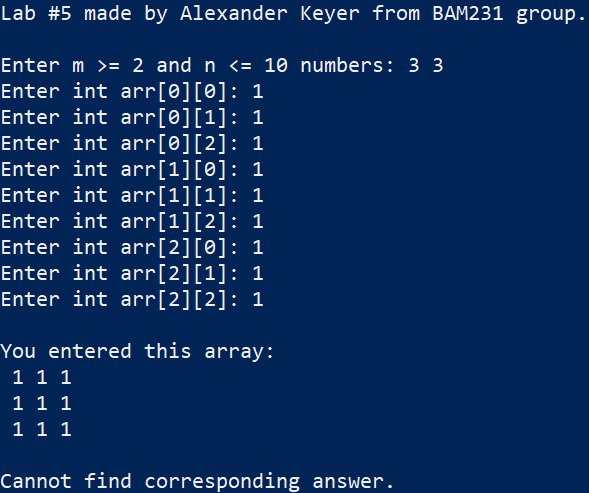
\includegraphics[width=400px]{test_3}
	Программа сработала корректно.
	
	\subsection*{Тест № 4}
	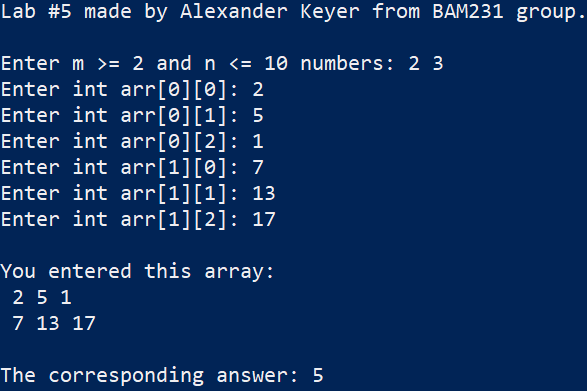
\includegraphics[width=400pt]{test_4}
	Программа сработала корректно.
	
\end{document}
